\documentclass[11pt,aspectratio=169,english]{beamer}

\usepackage{multirow}
\usepackage{mathpazo}
\usepackage{natbib}
\usepackage{setspace}
\usepackage{tikz}
\usepackage{babel}
\usepackage[utf8]{inputenc}
\usepackage[T1]{fontenc}
\usepackage{subcaption}
\usepackage{ragged2e}
\usepackage{color, colortbl}
\usepackage{xcolor}
\usepackage{mathptmx}
\usepackage{multirow}
\usepackage{FiraSans}

% Theme, color and font
% \usetheme{focus}
\usetheme{Singapore}
\usecolortheme{seagull}
% \usefonttheme{professionalfonts}
\beamertemplatenavigationsymbolsempty
\setbeamertemplate{frametitle}[default][left]

% Bibliography
\urlstyle{same}
% \addbibresource{references.bib}
\bibliographystyle{apa-good}

% Custom bibliography item
\setbeamertemplate{bibliography item}[triangle]

\setbeamerfont{title}{size=\huge, shape=\scshape\bfseries}
\setbeamerfont{subtitle}{size=\Large, shape=\scshape, parent=structure}
\setbeamerfont{author}{size=\Large, shape=\scshape}

\setbeamerfont{institute}{size=\large, shape=\scshape}
\setbeamerfont{date}{size=\large, shape=\scshape}

\setbeamerfont{sectiontitle}{size=\huge, series=\scshape\bfseries}
\setbeamerfont{frametitle}{size=\Large, shape=\scshape}

\setbeamerfont{footline}{size=\scriptsize}

\setbeamerfont{focusframe}{size=\huge, shape=\scshape}

\setbeamerfont{description item}{shape=\bfseries}

\setbeamerfont{caption name}{shape=\bfseries}

\setbeamerfont{bibliography item}{size=\small, shape=\scshape}
\setbeamerfont{bibliography entry author}{size=\small, shape=\scshape}
\setbeamerfont{bibliography entry title}{size=\small, series=\scshape\bfseries}
\setbeamerfont{bibliography entry location}{size=\small, shape=\scshape\normalfont}
\setbeamerfont{bibliography entry note}{size=\small, shape=\scshape\normalfont}

% Colors
\definecolor{urlcolor}{rgb}{0,.145,.698}
\definecolor{linkcolor}{rgb}{0,0,0}
\definecolor{citecolor}{rgb}{.12,.54,.11}
\definecolor{emphRed}{RGB}{229, 80, 57}

% Graphics path
\graphicspath{{../figures/}}

% Custom commands
\newcommand{\emphRed}[1]{\textcolor{emphRed}{#1}}

% Hyperref setup
\hypersetup{
	breaklinks=true,  % so long urls are correctly broken across lines
		colorlinks=true,
		urlcolor=urlcolor,
		linkcolor=linkcolor,
		citecolor=citecolor,
}

% Colors for table
\newcommand{\blue}[1]{\textcolor{blue}{#1}}

%:Title elements
\title{Product composition in \\ vertically integrated markets}
\subtitle{IO Summer Meetings 2025}
\author[Felipe Del Canto]{Felipe Del Canto}
\institute[]{Harvard University}
\date{July 23, 2025}

%:Document
\begin{document}

%:Title
\frame[plain]{\titlepage}

\section{Motivation}

\begin{frame}{\textbf{Motivation}}
	\begin{itemize}
		\item Consumer welfare depends on prices but also on product offerings.\vspace{1ex}
			\begin{itemize}
				\item Through variety (\# of products).\vspace{1ex}
				\item Or product composition (e.g, quality).
			\end{itemize}
		\vfill

		\item Thus, accounting for endogenous product decisions is relevant.\vspace{1ex}
			\begin{itemize}
				\item Analysis of mergers \citep{Fan2013,MazzeoEtAl2018}.\vspace{1ex}
				\item Responses to bailouts \citep{Wollmann2018}.\vspace{1ex}
				\item Collusion on product offerings \citep{Sullivan2020}.\vspace{1ex}
				\item Market structure in general \citep{FanYang2020}.\vspace{1ex}
				\item Vertical integration/Exclusivity agreements \citep{Lee2013}.
			\end{itemize}
	\end{itemize}
\end{frame}

\begin{frame}{\textbf{Research question}}
	\begin{itemize}
		\item Research on vertical integration (VI) has focused on different aspects.\vspace{1ex}
			\begin{itemize}
				\item Double marginalization and foreclosure of rivals \citep{CrawfordEtAl2018}.\vspace{1ex}
				\item Access to \textit{existing} products and indirect network effects \citep{Lee2013}.
			\end{itemize} 
		\vfill

		\item However, in certain industries we could expect effects on the distribution of \vspace{1ex}
			\begin{enumerate}
				\item Horizontal characteristics.\vspace{1ex}
				\item Quality.
			\end{enumerate}
		\vfill

		\item This project attempts to understand effect of VI on both.\vspace{1ex}
			\begin{itemize}
				\item In the market for (digital) PC videogames.
			\end{itemize}
	\end{itemize}
\end{frame}

\section{Intuition and basic mechanisms}

\begin{frame}{\textbf{Overview of the production process} \hypertarget{industryOverviewBack}{}} 
	\begin{itemize}
		\item Game developers create games.\vspace{1ex}
			\begin{itemize}
				\item But (usually) need a publisher.\vspace{1ex}
				\item To handle marketing, distribution, funding and others. \citep{GilWarzynski2015}
			\end{itemize}
		\vfill

		\item Finally, games are sold on stores.\vspace{1ex}
			\begin{itemize}
				\item Today, mostly digital (89.5\% in 2022).
			\end{itemize}
		\vfill

		\item Currently, these engage in complex vertical relationships. \hyperlink{verticalDiagram}{\beamerbutton{Diagram}}
	\end{itemize}
\end{frame}

\begin{frame}{\textbf{Why could VI impact quality?}}
	\begin{itemize}
		\item Publishers fundamentally provide three services to developers\vspace{1ex}
			\begin{enumerate}
				\item Financing.\vspace{1ex}
				\item Quality assurance.\vspace{1ex}
				\item Marketing/advertising.
			\end{enumerate}
		\vfill
		
		\item The first two can improve quality directly.\vspace{1ex}
			\begin{itemize}
				\item Financing allows developers to invest more in the game.\vspace{1ex}
				\item Quality assurance can help avoid bugs and improve user experience.
			\end{itemize}
		\vfill

		\item Marketing can improve the \textit{perceived} quality.
	\end{itemize}
\end{frame}

\begin{frame}{\textbf{How can VI impact horizontal differentiation?}}
	\begin{itemize}
		\item Choice of which developer(s) to acquire is \textit{endogenous}.
		\vfill

		\item If products are substitutable: VI $\Rightarrow$ better profitability $\Rightarrow$ forclosure.\vspace{1ex}
			\begin{itemize}
				\item This could affect products far away in characteristics space. 
			\end{itemize}
		\vfill

		\item However, publishers might also want to diversify their offerings.\vspace{1ex}
			\begin{itemize}
				\item To avoid risk and to reach different audiences.\vspace{1ex}
				\item This could lead to more products in the market.
			\end{itemize}
	\end{itemize}
\end{frame}

\section{Next steps}

\begin{frame}{\textbf{Next steps}}
	\begin{itemize}
		\item Collect data.\vspace{1ex}
			\begin{itemize}
				\item Game data and historical prices can be obtained directly from Steam.\vspace{1ex}
				\item Sales data can be purchased from VG Insights.
			\end{itemize}
		\vfill

		\item Think thoroughly about a model and relevant counterfactuals.
	\end{itemize}
\end{frame}

\appendix

\begin{frame}[plain,c]
	\begin{center}
		\vspace{5ex}
		\Huge\bf THANK YOU!
	\end{center}
\end{frame}


\begin{frame}[allowframebreaks, plain]
	\frametitle{\bf References}
	\def\newblock{\hskip .11em plus .33em minus .07em}
	\bibliography{../../references.bib}
\end{frame}

\appendix

\section{Appendix: Industry details}

\begin{frame}[plain]{\textbf{The videogame industry is sizable}}
	\begin{figure}[H]
		\centering
		\begin{subfigure}{0.48\textwidth}
			\includegraphics[width=\textwidth]{revenueByType2023.png}
		\end{subfigure} \hfill
		\begin{subfigure}{0.48\textwidth}
			\includegraphics[width=\textwidth]{revenueTopCompanies.png}
		\end{subfigure}

		\caption{Source: Newzoo (2023)}
	\end{figure}
\end{frame}

\begin{frame}[plain]{\textbf{Recent trends in vertical integration}}
	\begin{itemize}
		\item Important trend in acquisitions by large companies.
		\vfill
		\item Since 2020, Microsoft spent more than \$80bn in acquisitions.\vspace{1ex}
		\begin{itemize}
			\item \$7.5bn in 2020 for Zenimax.\vspace{1ex}
			\item \$75.4bn in 2023 for Activision-Blizzard(-King).
		\end{itemize}
		\vfill

		\item Sony has also acquired 11 developers since 2021.\vspace{0.5ex}
		\begin{itemize}
			\item Biggest acquisition was Bungie for \$3.7bn.
		\end{itemize}
		
	\end{itemize}
\end{frame}

\begin{frame}[plain]{\textbf{Why the market for PC videogames}}
	\begin{itemize}
		\item PC is multipurpose so (lifetime) value is not just due to games.\vspace{1ex}
			\begin{itemize}
				\item Alleviates demand system complexity.
			\end{itemize} 
		\vfill

		\item Publishers and developers are not hardware manufacturers.\vspace{1ex}
			\begin{itemize}
				\item No concern about platform incentives.
			\end{itemize}
		\vfill

		\item Also... it is the data that I can get (for now!).
	\end{itemize}
\end{frame}

\section{Data}

\begin{frame}[plain]{\textbf{Data}}
	\begin{itemize}
		\item Data from PC games sold on Steam.\vspace{1ex}
			\begin{itemize}
				\item Biggest digital distribution platform ($\sim$\$9bn in sales vs $\sim$\$1bn on Epic Store).
			\end{itemize}
		\vfill 

		\item Publicly available data. \vspace{1ex}
			\begin{itemize}
				\item Game characteristics (e.g., genre, historical prices, release date).\vspace{1ex}
				\item Developer and publisher information.
			\end{itemize}
		\vfill

		\item Can also obtain developer ownership from multiple sources.
	\end{itemize}
\end{frame}

\begin{frame}[plain]{\textbf{Data}}
	\begin{itemize}
		\item VG Insights also has rich (proprietary) data on games sold on Steam.
		\vfill

		\item Daily data on sales and prices for each game since 2014.
		\vfill
		
		\item Also breakdown of total sales by region.\vspace{1ex}
			\begin{itemize}
				\item For a subset of games.
			\end{itemize} 

	\end{itemize}
\end{frame}

\begin{frame}[plain]{\textbf{Complex vertical market} \hyperlink{industryOverviewBack}{\beamerbutton{Back to industry}}} \hypertarget{verticalDiagram}{} 
	\begin{figure}[H]
		  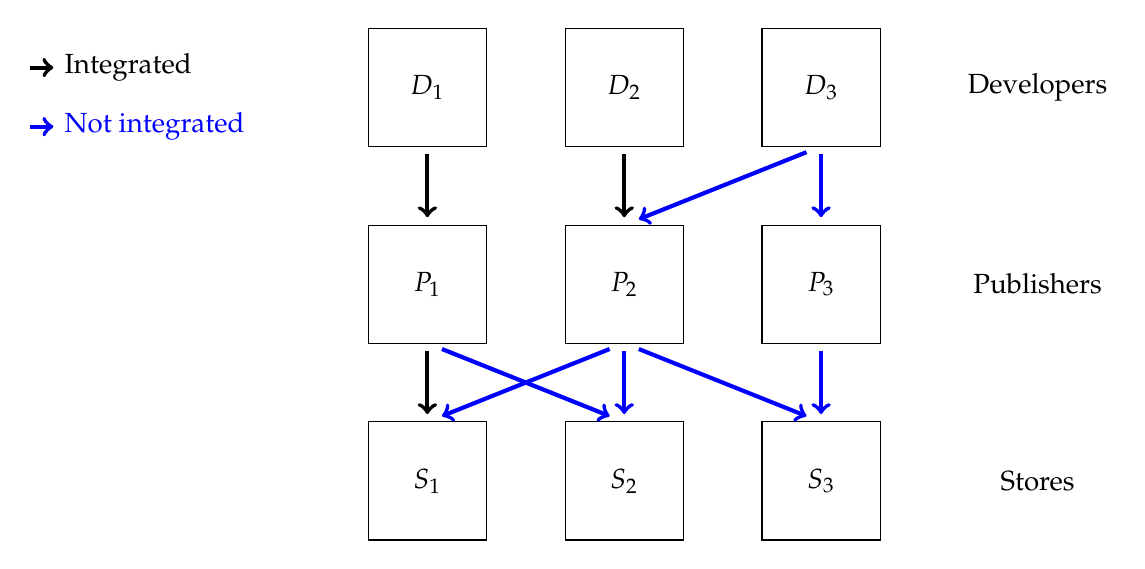
\begin{tikzpicture}
			% Developers
			\begin{scope}[local bounding box=d1]
				\draw (0,5) rectangle (1.5,6.5) node[pos=.5] {$D_{1}$};
			\end{scope}
			\begin{scope}[local bounding box=d2]
				\draw (2.5,5) rectangle (4,6.5) node[pos=.5] {$D_{2}$};
			\end{scope}
			\begin{scope}[local bounding box=d3]
				\draw (5,5) rectangle (6.5,6.5) node[pos=.5] {$D_{3}$};
			\end{scope}

			 \node at (8.5,5.75) {Developers};

			% Publishers
			\begin{scope}[local bounding box=p1]
				\draw (0,2.5) rectangle (1.5,4) node[pos=.5] {$P_{1}$};
			\end{scope}
			\begin{scope}[local bounding box=p2]
				\draw (2.5,2.5) rectangle (4,4) node[pos=.5] {$P_{2}$};
			\end{scope}
			\begin{scope}[local bounding box=p3]
				\draw (5,2.5) rectangle (6.5,4) node[pos=.5] {$P_{3}$};
			\end{scope}

			\node at (8.5,3.25) {Publishers};

			% Stores
			\begin{scope}[local bounding box=s1]
				\draw (0,0) rectangle (1.5,1.5) node[pos=.5] {$S_{1}$};
			\end{scope}
			\begin{scope}[local bounding box=s2]
				\draw (2.5,0) rectangle (4,1.5) node[pos=.5] {$S_{2}$};
			\end{scope}
			\begin{scope}[local bounding box=s3]
				\draw (5,0) rectangle (6.5,1.5) node[pos=.5] {$S_{3}$};
			\end{scope}

			\node at (8.5,0.75) {Stores};

			% Arrows from developers to publishers
			% Can use \uncover<n-m>{} to show in specific slides
			
			\uncover<2->{\draw[->, shorten >=1mm, shorten <=1mm, line width=1.5pt] (d1) -- (p1);}
			\uncover<3->{\draw[->, shorten >=1mm, shorten <=1mm, line width=1.5pt] (d2) -- (p2);}

			\uncover<3->{\draw[->, shorten >=2mm, shorten <=2mm, line width=1.5pt, color=blue] (d3.south) -- (p2.north);}
			\uncover<3->{\draw[->, shorten >=1mm, shorten <=1mm, line width=1.5pt, color=blue] (d3) -- (p3);}

			% Arrows from publishers to stores
			\uncover<2->{\draw[->, shorten >=1mm, shorten <=1mm, line width=1.5pt] (p1) -- (s1);}
			\uncover<3->{\draw[->, shorten >=2mm, shorten <=2mm, line width=1.5pt, color=blue] (p1.south) -- (s2.north);}

			\uncover<3->{\draw[->, shorten >=2mm, shorten <=2mm, line width=1.5pt, color=blue] (p2.south) -- (s1.north);}
			\uncover<3->{\draw[->, shorten >=1mm, shorten <=1mm, line width=1.5pt, color=blue] (p2.south) -- (s2.north);}
			\uncover<3->{\draw[->, shorten >=2mm, shorten <=2mm, line width=1.5pt, color=blue] (p2.south) -- (s3.north);}

			\uncover<3->{\draw[->, shorten >=1mm, shorten <=1mm, line width=1.5pt, color=blue] (p3) -- (s3);}

			% Legend
			\uncover<2->{\draw [->, line width=1.5pt] (-4.3, 6) -- (-4, 6) node[right] {Integrated};}
			\uncover<3->{\draw [->, line width=1.5pt, color=blue] (-4.3, 5.25) -- (-4, 5.25) node[right] {Not integrated};
			}

		\end{tikzpicture}
	\end{figure}
\end{frame}

\begin{frame}[plain]{\textbf{Revenue breakdown by region}}
	\begin{figure}[H]
		\centering
		\includegraphics[width=0.75\textwidth]{revenueByRegion.png}
		\caption{Source: Newzoo (2023)}
	\end{figure}
\end{frame}

\begin{frame}[plain]{\textbf{People are playing more}}

	\begin{figure}[H]
		\centering
		\includegraphics[width=0.7\textwidth]{playersByYear.jpeg}
		\caption{Source: Newzoo (2020)}
	\end{figure}

\end{frame}

\begin{frame}[plain]{\textbf{Important move towards services}}

	\begin{itemize}
		\item For EA alone, \$1.7B in revenue from transactions in live service games in 2023Q3. 
		\vfill
		\item 95\% of studios working on or planning to release a live service (Griffin, 2023).
		\vfill
		
		\item Important concerns about addiction and gambling.\vspace{1ex}
			\begin{itemize}
				\item This has led to a number of lawsuits recently. 
			\end{itemize}
	\end{itemize}

\end{frame}

\begin{frame}[plain]{\textbf{Some videogames are comparable to films}}

	\begin{itemize}
		\item High-budget (AAA) games have similar budgets and production times as films.\vspace{0.5ex}
		\begin{itemize}
			\item But success may vary.
		\end{itemize}
	\end{itemize}

	\begin{table}[H]
		\caption{Budgets and revenues of AAA games and high grossing films.}

		\begin{tabular}{lcccc}
			\textbf{Title}   &  \textbf{Year}   &   \textbf{Budget}  & \textbf{Revenue}   & $\frac{\textbf{Revenue}}{\textbf{Budget}}$ \\[0.5ex] \hline
			\\[-1.5ex]
			\blue{Horizon Forbidden West} & \blue{2022} & \blue{212M} & \blue{588M} & \blue{2.77} \\[0.5ex]
			Avatar: The Way of Water & 2022 & 350-460M & 2.3B & 5.00-6.57 \\[0.5ex]
			\blue{The Last of Us Part II} & \blue{2020} & \blue{220M} & \blue{700M} & \blue{3.18} \\[0.5ex]
			Avengers: Endgame & 2019 & 356-400M & 2.8B & 7.00-7.87 \\[0.5ex]
		\end{tabular}
	\end{table}
\end{frame}

\begin{frame}[plain]{\textbf{A quote from a VP of King} \hyperlink{modelSupplyDev}{\beamerbutton{Back to Developers}}} \hypertarget{quoteVPKing}{}

	\begin{spacing}{1.5}
	``In the mature phase (...) [t]he focus for the company is most likely on \emphRed{serving the existing loyal audience, rather than attracting a new one}. (...) If you've made it this far, you most likely have a very deep understanding of the audience you are serving with your successful game(s), what makes them tick and what will make them open their wallets.''\\
	{\raggedleft - Kim Nordstrom, VP at King. \par}
	\end{spacing}

\end{frame}



\end{document}

